\section{Robot Design}
% describe the design
% what are the advantages
We mainly focus on two aspects when configuring the Lego robot, namely {\itshape \rom{1})} stability and {\itshape \rom{2})} feasibility. The complete configuration of the robot is visualised in Fig.\ref{fig:robotconfig}, where there are three images showing the front, side and back appearances of the robot respectively. 

The total height of the robot is approximately 18 cm. The width and length are 13 cm and 19.5 cm, respectively. This configuration ensures that the robot does not occupy too much space in the arena. The ultrasonic sensor is placed in the lower front with an approximate height of 6.5 cm and has a vision range of 180 degrees. A previous prototype with the sensor on the top and 360 degrees of freedom was tested but the wire connected to de brick interfered the sensor spin. A novel feature used in this design is the support device installed in the back as shown in Fig.\ref{fig:backrobot}, where two balls are positioned inside the two white slots to reduce the friction between the ground and the support device while rotating and moving. 

\begin{figure}[h]
\centering
  \begin{subfigure}{0.25\textwidth}
  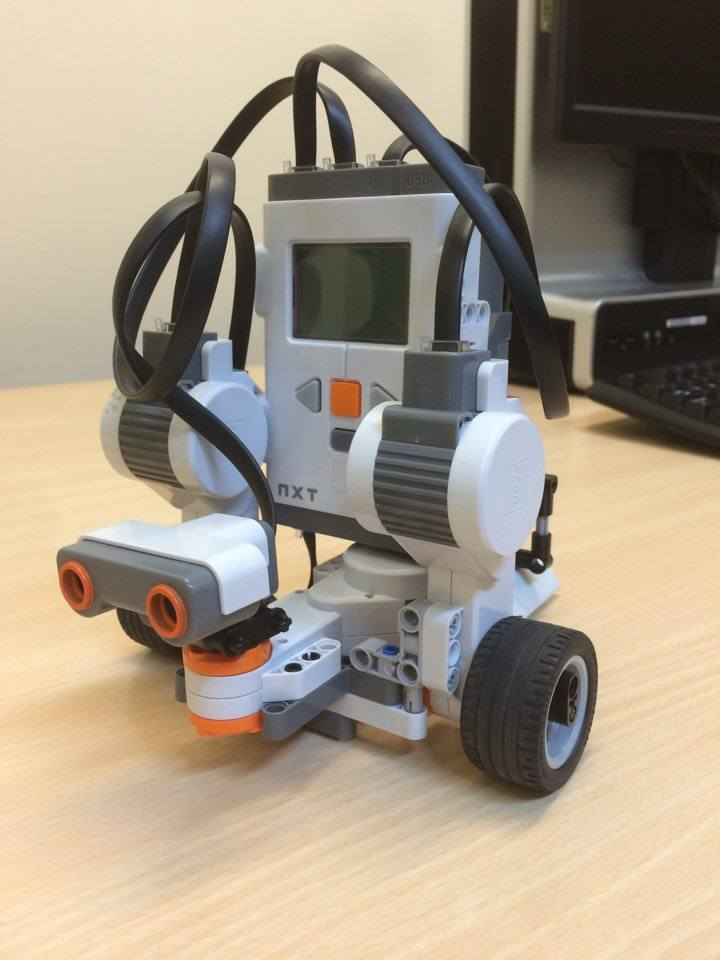
\includegraphics[scale=0.15]{f}
  \caption{Front appearance}
  \end{subfigure}
  \begin{subfigure}{0.25\textwidth}
  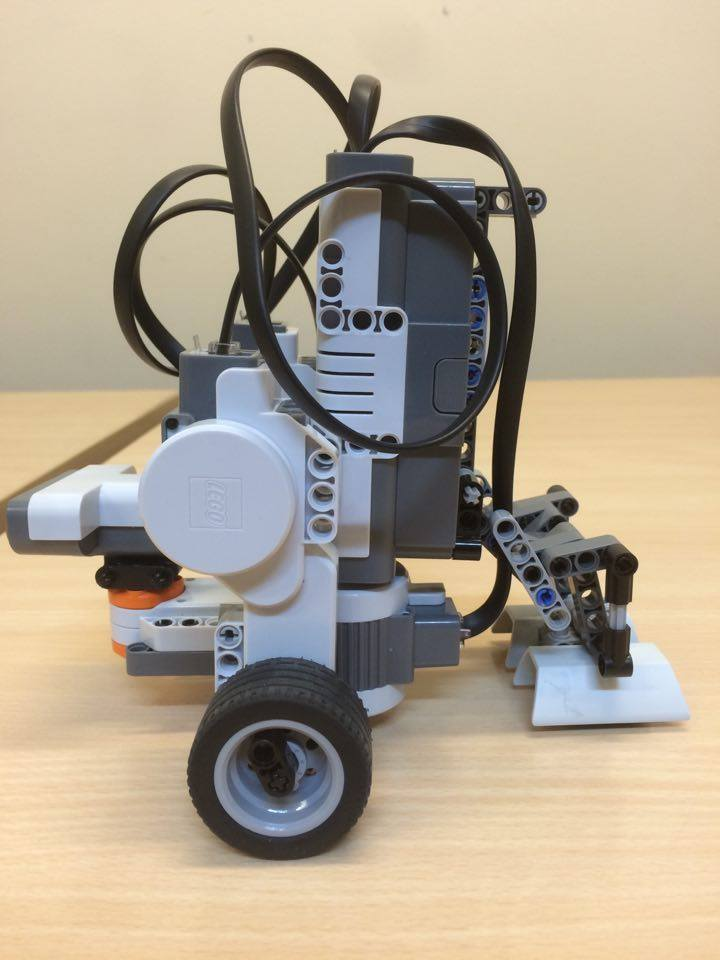
\includegraphics[scale=0.15]{s}
  \caption{Side appearance}
  \end{subfigure}
  \begin{subfigure}{0.25\textwidth}
  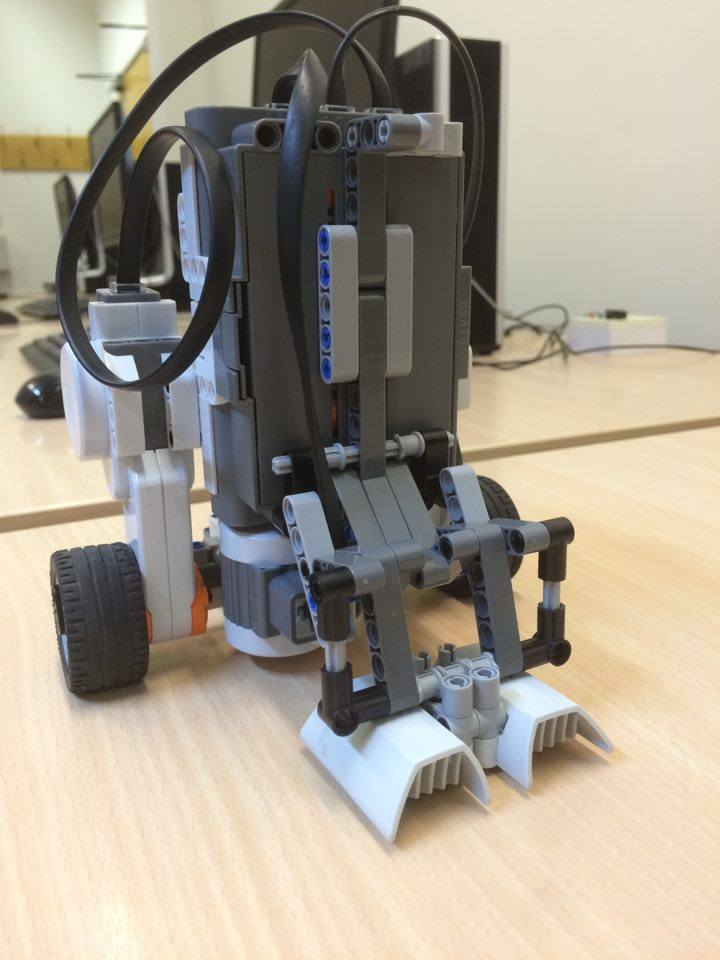
\includegraphics[scale=0.15]{b}
  \caption{Back appearance} \label{fig:backrobot}
  \end{subfigure}
  \caption{Robot configuration.}
  \label{fig:robotconfig}
\end{figure}

\subsection{Sensors}

Our robot only uses the ultrasonic sensor to measure the environment. In Fig.\ref{fig:sensorerrors}, the dense blue points represent the roughly accurate sensor readings. The red points away from the blue lines are the invalid readings that are caused by corners. Therefore, it can be concluded that the ultrasonic sensor cannot perform well in measuring the distance from corners and the resulting readings are thus outliers that should be discarded.

In order to discard those outliers, after receiving all the information from the environment, the scan range is divided into sections based on the difference between the neighbouring datapoints, for example, Fig.\ref{fig:err2} is divided into 3 sections. To determine between real walls and noise a rule considers the angle from the first point (rightmost/bottom) in the section to the last point (leftmost/top) in the same section taking as the origin the coordinate (0,0), if the resulting angle is less than 15 degrees then that section is considered as noise. 

\begin{figure}[h]
\centering
	\begin{subfigure}{0.5\textwidth}
		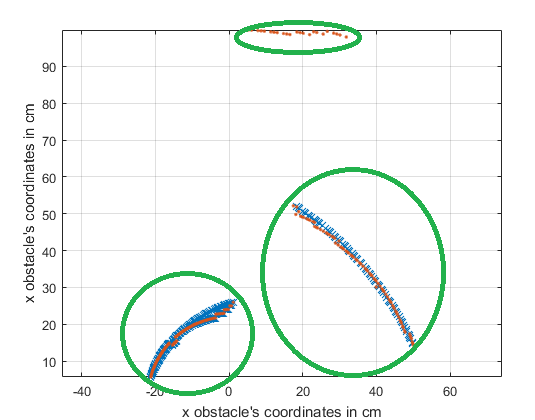
\includegraphics[scale=0.50]{noCorners1}
		\caption{Robot standing perpendicular to a corner}
		\label{fig:err2}
	\end{subfigure}
	\begin{subfigure}{0.4\textwidth}
		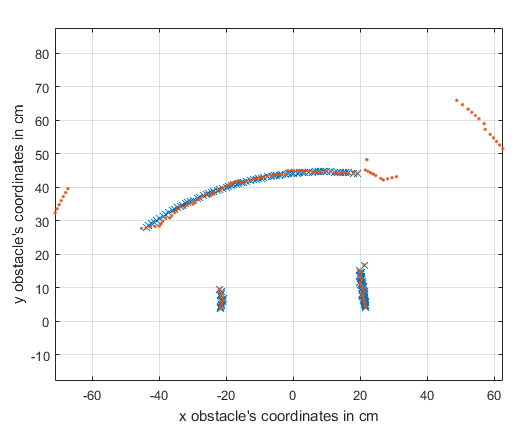
\includegraphics[scale=0.50]{noCorners2}
		\caption{Robot standing in front of a wall and one on each side}
	\end{subfigure}
	\caption{Sensor error.}
	\label{fig:sensorerrors}
\end{figure}
\FloatBarrier
